\documentclass[12pt]{article}%
\usepackage{amsfonts}
\usepackage{fancyhdr}
\usepackage{comment}
\usepackage[a4paper, top=2.5cm, bottom=2.5cm, left=2.2cm, right=2.2cm]%
{geometry}
\usepackage{times}
\usepackage{amsmath}
\usepackage{listings}
\usepackage{changepage}
\usepackage{amssymb}
\usepackage{graphicx}%
\usepackage{amsmath} 
\setcounter{MaxMatrixCols}{30}
\newtheorem{theorem}{Theorem}
\newtheorem{acknowledgement}[theorem]{Acknowledgement}
\newtheorem{algorithm}[theorem]{Algorithm}
\newtheorem{axiom}{Axiom}
\newtheorem{case}[theorem]{Case}
\newtheorem{claim}[theorem]{Claim}
\newtheorem{conclusion}[theorem]{Conclusion}
\newtheorem{condition}[theorem]{Condition}
\newtheorem{conjecture}[theorem]{Conjecture}
\newtheorem{corollary}[theorem]{Corollary}
\newtheorem{criterion}[theorem]{Criterion}
\newtheorem{definition}[theorem]{Definition}
\newtheorem{example}[theorem]{Example}
\newtheorem{exercise}[theorem]{Exercise}
\newtheorem{lemma}[theorem]{Lemma}
\newtheorem{notation}[theorem]{Notation}
\newtheorem{problem}[theorem]{Problem}
\newtheorem{proposition}[theorem]{Proposition}
\newtheorem{remark}[theorem]{Remark}
\newtheorem{solution}[theorem]{Solution}
\newtheorem{summary}[theorem]{Summary}
\newenvironment{proof}[1][Proof]{\textbf{#1.} }{\ \rule{0.5em}{0.5em}}
\usepackage{color}

\definecolor{dkgreen}{rgb}{0,0.6,0}
\definecolor{gray}{rgb}{0.5,0.5,0.5}
\definecolor{mauve}{rgb}{0.58,0,0.82}

\lstset{frame=tb,
  language=MATLAB,
  aboveskip=3mm,
  belowskip=3mm,
  showstringspaces=false,
  columns=flexible,
  basicstyle={\small\ttfamily},
  numbers=none,
  numberstyle=\tiny\color{gray},
  keywordstyle=\color{blue},
  commentstyle=\color{dkgreen},
  stringstyle=\color{mauve},
  breaklines=true,
  breakatwhitespace=true,
  tabsize=3
}

\newcommand{\Q}{\mathbb{Q}}
\newcommand{\R}{\mathbb{R}}
\newcommand{\C}{\mathbb{C}}
\newcommand{\Z}{\mathbb{Z}}

\begin{document}

\title{Project 1}
\author{Shad Mahmod \\
Modelling Complex Systems}
\date{\today}
\maketitle
\section{A firing brain}

In this part a model of cellular automata was implemented on a NxN grid on which the boundaries were periodic, e.g. the rightmost end of the grid connected to the leftmost grid.
 

\subsection{}
In figure \ref{fig:mesh1} we see the inital mesh. The colors \{blue, green, yellow\} correspond to the states \{ready, firing, resting\} in the corresponding order. In figure \ref{fig:mesh2} the state of the grid at the iterations \{10, 20, 100, 1000\} are shown.
\begin{figure}[htbp]
    \centering
    \includegraphics[scale=0.3]{Pictures/initial.jpg}
    \caption{The initial state of the cells}
    \label{fig:mesh1}
\end{figure}

\begin{figure}[htbp]
    \centering
    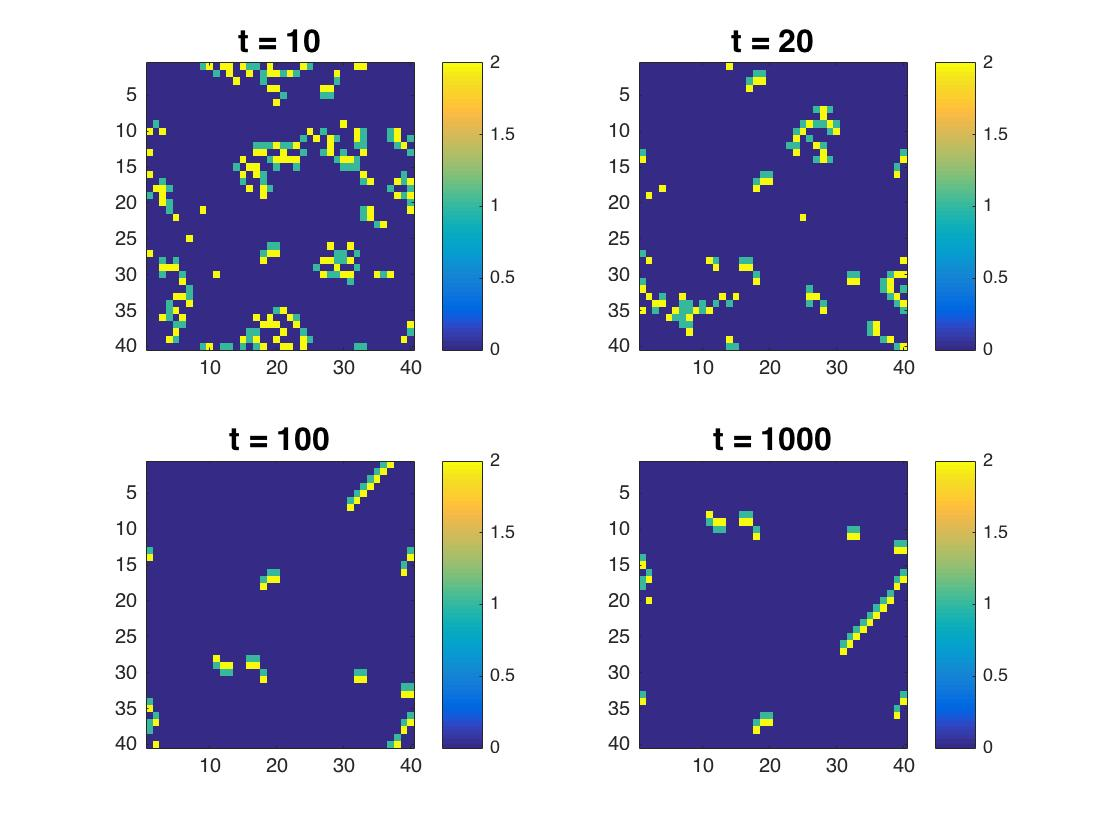
\includegraphics[scale=0.4]{Pictures/Simul1020.jpg}
    \caption{The grid at different timesteps}
    \label{fig:mesh2}
\end{figure}
Even though the initial state of the system consists of \textit{firing}, after only then iterations this number is significantly reduced. At $t=10$ the system have started to converge towards some patches of firing and resting cells. At $t=\{20, 100, 1000\}$ the trend seems to continue where the patches, or groups, of cells are reduced.
\begin{figure}[htbp]
    \centering
    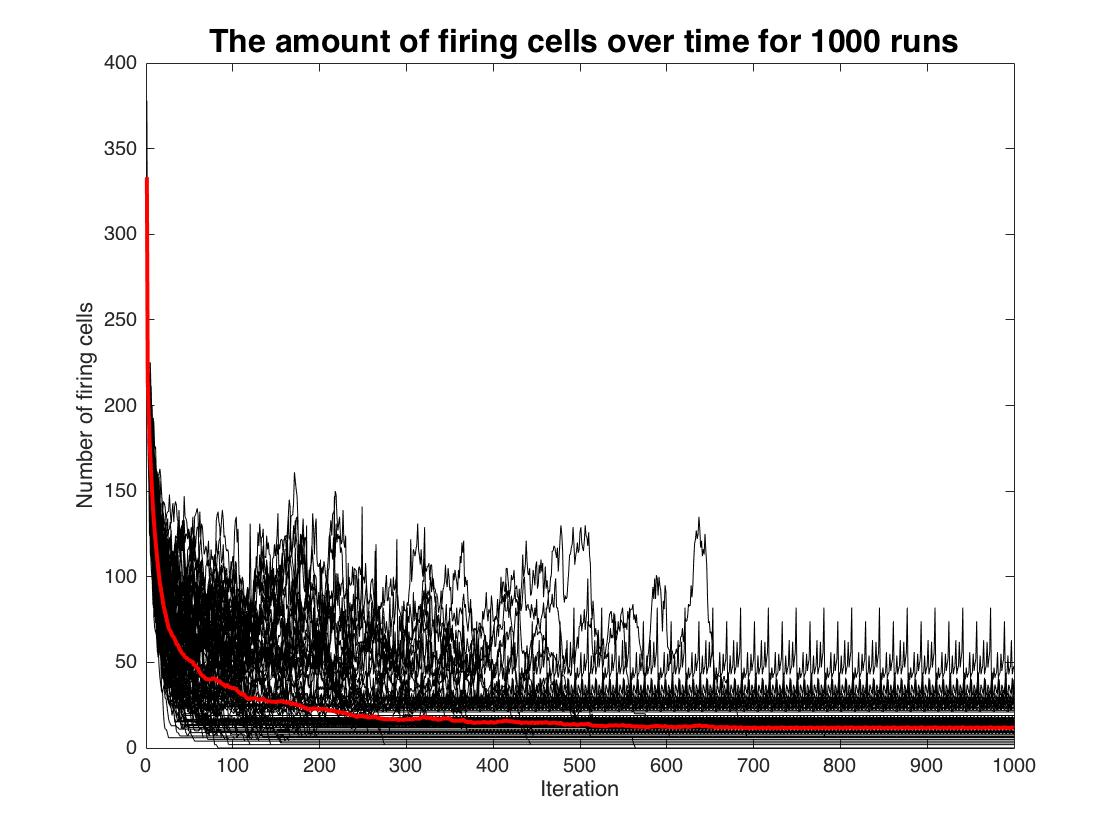
\includegraphics[scale=0.4]{Pictures/Aver1000.jpg}
    \caption{A graph showing the number of cells in firing state for 100 runs over 1000 timesteps. The red line is the average amount of firing cells at each timestep.}
    \label{fig:mesh3}
\end{figure}
\\�\\
In figure \ref{fig:mesh3} the system was spawned 100 times and each time allowed to run for 1000 iterations. The black lines are the sums of cells in firing state for different runs and the red line is the average number of firing cells at each iteration. From the figure it is evident that the amount of firing cells fluctuates a lot but decreases over time. After around 650 iterations, all of the systems had entered an equilibrium state in which the system had converged towards 0 firing cells, a constant amount of firing cells or (most likely) a fluctuating amount of firing cells. From figure \ref{fig:mesh3} it can be noted that in none of the simulations is the amount of firing cells after iteration 650 more than 100.


\subsection {}
\subsubsection{}
The shape seen in figure \ref{fig:mesh5} moves downwards with a rate of one step per iteration.

\begin{figure}[htbp]
    \centering
        \caption{A shape that moves 1 step per timeunit and doesn't change form.}

    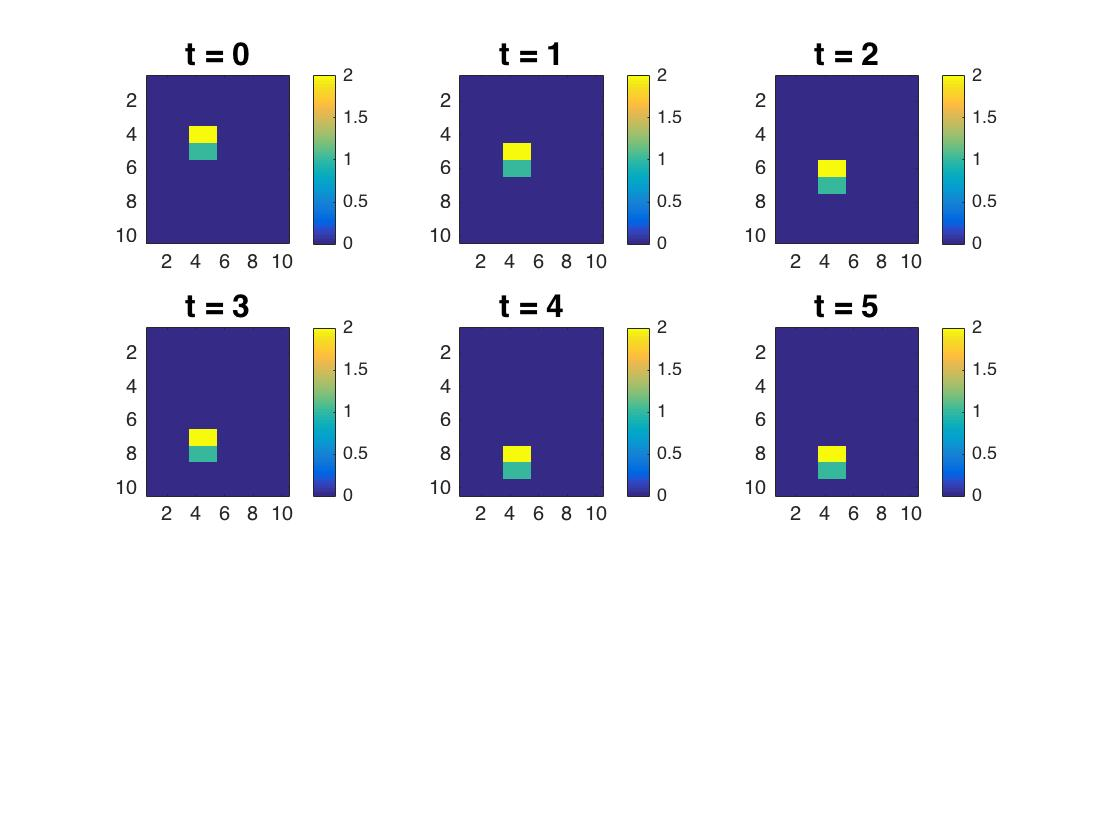
\includegraphics[scale=0.3]{Pictures/OneCellMover.jpg}
    \label{fig:mesh5}
\end{figure}
\subsubsection{}
In the top left picture of figure \ref{fig:sooter} we have a group of cells who will move upwards with one step per time unit and will simultaneously shoot out a cell downwards as seen in the other subplots of the same figure.

\begin{figure}[htbp]
    \centering
    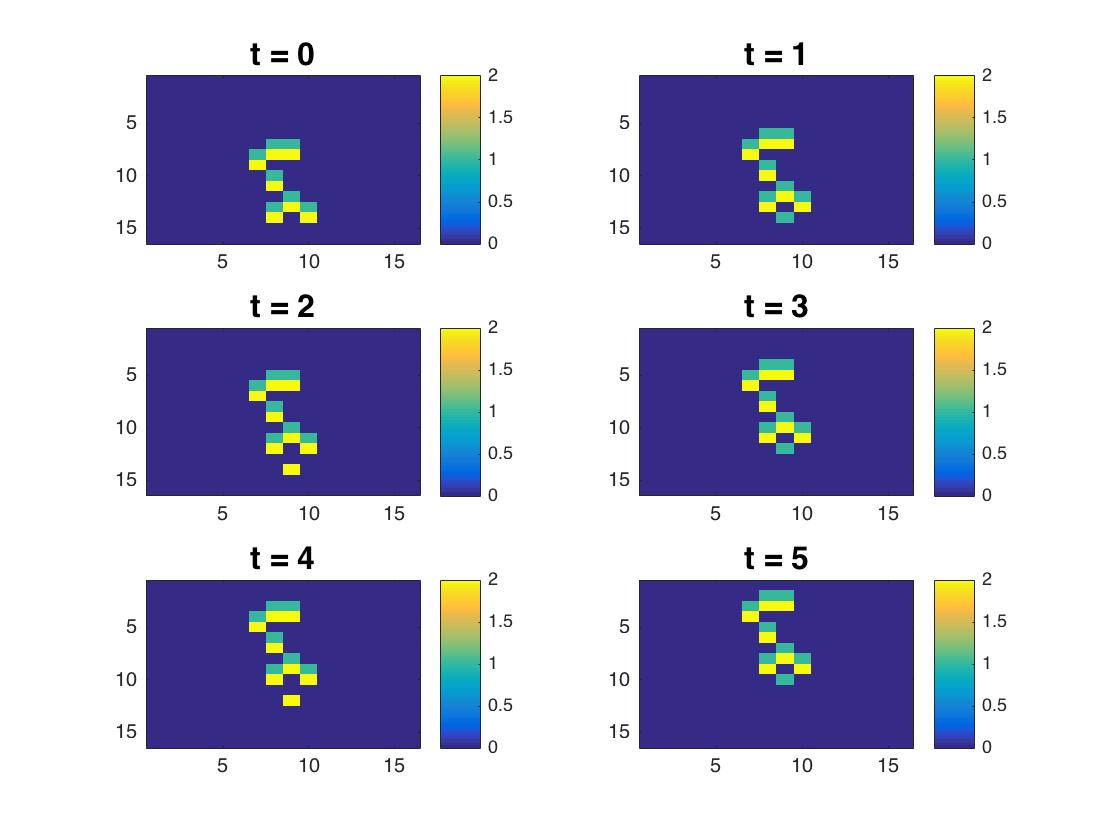
\includegraphics[scale=0.3]{Pictures/Leav1.jpg}
    \caption{A group of cells that move 1 step/iteration and leave behind a cell.}
    \label{fig:sooter}
\end{figure}

\subsubsection{}
The shape seen in figure \ref{fig:mesh6a} is periodic and after three time steps it returns to the same shape at the same location. The whole shape has moved two units to the right and one unit upwards during these 4 iterations, thus it moves slower than one cell per iteration on average.
\begin{figure}[htbp]
    \centering

    \includegraphics[scale=0.3]{Pictures/perMov.jpg}
            \caption{A shape that returns to it's form after 4 timesteps and has moved.}

    \label{fig:mesh6a}
\end{figure}
\subsubsection{}
The shape seen in figure \ref{fig:osc} is stationary but oscillates periodically.
\begin{figure}[htbp]
    \centering

    \includegraphics[scale=0.3]{Pictures/perMov.jpg}
            \caption{A shape that returns to it's form after 4 timesteps.}

    \label{fig:osc}
\end{figure}
\subsubsection{}

\subsection{Custom system}
In this system the cells can be in four different states \textit{\{null, prey, hunter, hunterkiller\}}. For any cell, the number of neighboring null-cells is denoted $N_n$, the number of prey-cells $N_p$ and so on. We have the following transitions. 

\begin{align*} 
Null & \Rightarrow  \left\{
  \begin{array}{@{}ll@{}}
    Prey \text{ with probability } P_{N2P}(N_p) & \text{if}\ N_h = 0 \ and \ N_p \neq 0 \\
    Hunter \text{ with probability } P_{N2H}(N_h) & \text{if}\ N_h \neq 0  \\
  \end{array}\right.\\ 
  Hunter & \Rightarrow  \left\{
  \begin{array}{@{}ll@{}}
    Hunterkiller \text{ with } P_{H2HK}(N_{hk}) & \text{if}\ N_{hk} \neq 0  \\
    Null \text{ with } P_{H2N} = 0.1 & \text{if}\ N_{n} \geq 6  \\
    Null \text{ with } P_{H2N} = 0.001
  \end{array}\right.\\ 
  Prey & \Rightarrow  \left\{
  \begin{array}{@{}ll@{}}
    Hunter \text{ with probability } P_{P2Hk}=\text{if}\ N_h \neq 0 \\
    Hunterkiller \text{ with probability } P_{N2H}(N_h) & \text{if}\ N_h \neq 0  \\
    Null  \text{ with P = 0.03 if }\ N_p > 5 \text{ and } N_h \neq 0  
  \end{array}\right.\\ 
  Hunterkiller & \Rightarrow  \left\{
  \begin{array}{@{}ll@{}}
    Prey \text{ with } P_{HK2P}=0.3 & \text{if surrounded by hunterkillers and preys}  \\
  \end{array}\right.\\ 
\end{align*}
where
\begin{align*} 
P_{N2P} & =  \left\{
  \begin{array}{@{}ll@{}}
    0.03 & \text{if}\ N_p = 1  \\
    0.06 & \text{if}\ N_p = 2  \\
    0.09 & \text{if}\ N_p = 3  \\
    0.12 & \text{if}\ N_p = 4  \\
    0.16 & \text{if}\ N_p = 5  \\
    0.2 & \text{if}\ N_p = 6  \\
    0.25 & \text{if}\ N_p = 7  \\
    0.30 & \text{if}\ N_p = 8  \\
  \end{array}\right. & P_{N2H} & =  \left\{
  \begin{array}{@{}ll@{}}
    0.03 & \text{if}\ N_h = \{0, 1, 2\}  \\
    0.02 & \text{if}\ N_p = \{3, 4, 5\}  \\
    0.01 & \text{if}\ N_p = \{6, 7, 8\}  \\
  \end{array}\right. \\ 
\end{align*}
   \begin{align*} 
P_{H2HK} & =  \left\{
  \begin{array}{@{}ll@{}}
    0.5 & \text{if}\ N_{hk} = 1  \\
    0.75 & \text{if}\ N_{hk} = 2  \\
    0.8 & \text{if}\ N_{hk} = 3  \\
    0.9 & \text{if}\ N_{hk} = 4  \\
    0.95 & \text{if}\ N_{hk} = 5  \\
    0.1 & \text{if}\ N_{hk} = \{6, 7, 8\}  \\
  \end{array}\right. & P_{P2H} & =  (1-\frac{N_n}{8})\left\{
  \begin{array}{@{}ll@{}}
    0.3 & \text{if}\ N_h = 1  \\
    0.4 & \text{if}\ N_h =2  \\
    0.5 & \text{if}\ N_h = 3  \\
    0.6 & \text{if}\ N_h = 4  \\
    0.7 & \text{if}\ N_h = 5  \\
    0.8 & \text{if}\ N_h = 6  \\
    0.9 & \text{if}\ N_h = 7  \\
    0.1 & \text{if}\ N_h = 8  \\
  \end{array}\right. \\ 
\end{align*}                   
\subsubsection{Random run}
We run a simulation by initializing a system in which is 100x100 cells in size and a cell is initialized to:
    \begin{align*} 
Cell & =  \left\{
  \begin{array}{@{}ll@{}}
    Null & \text{with}\ P = 0.9  \\
    Hunter & \text{with}\ P = 0.075  \\
    Prey & \text{with}\ P = 0.02  \\
    Hunterkiller & \text{with}\ P = 0.005  \\
  \end{array}\right.
   \end{align*}
   
The initial state of the system is seen in figure \ref{fig:cInit1}. The colors \{black, red, yellow, green\} correspond \{null, hunter, prey, hunterkiller\}. In figure \ref{fig:cInit} the system is shown at timesteps \{10, 30, 60, 100\}. A video of the simulation is available online.\footnote{https://vimeo.com/263155236} At timestep 10 it is seen that the amount of prey cells (yellow in the figure) have grown the most whereas there is only a slight increase in hunterkiller cells (green in the figure). \\ \\
At timestep 30, the prey cells have formed a more robust and connected state. Since they are taking up such a large part of the grid they are more susceptible to being attacked by hunters, which is the reason to why there are some large patches of hunter cells (red in the figure). The increase in hunter cells also brings an increase in hunterkiller cells, since these prey on hunter cells. Therefore we see some slightly smaller patchs of hunterkiller cells.\\�\\
In the two final subplots the system is cleared of large patches of hunter cells but we do have some spread out cells and the at each timestep some new hunter cells might spawn. More interestingly, we see that at the borders of the infrastructure that consists of prey cells, there are green cells. These green cells have thus created a defensive perimeter to protect the prey structure. against external \textit{attacks}.           
\begin{figure}[htbp]
    \centering
    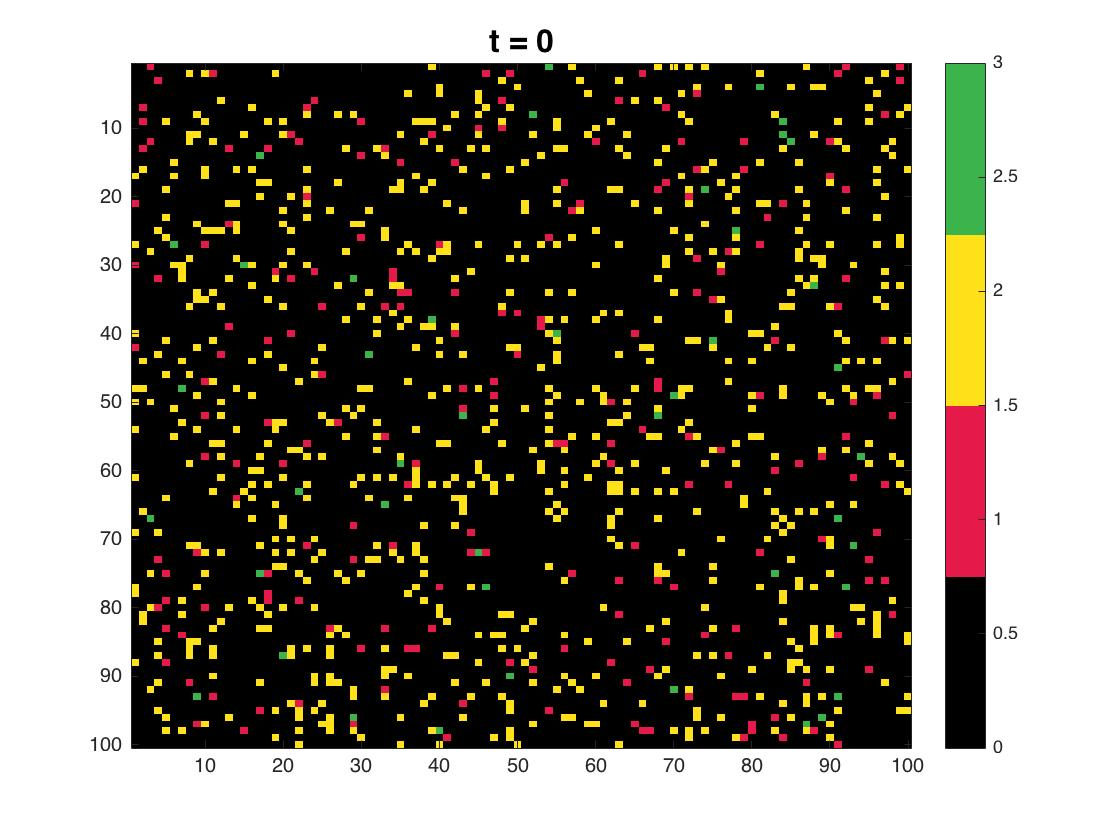
\includegraphics[scale=0.3]{Pictures/cInit1.jpg}
    \caption{A grid of the cells at the systems initial state. Here the colors \{black, red, yellow, green\} correspond \{null, hunter, prey, hunterkiller\}}
    \label{fig:cInit1}
\end{figure}                      
  \begin{figure}[htbp]
    \centering
    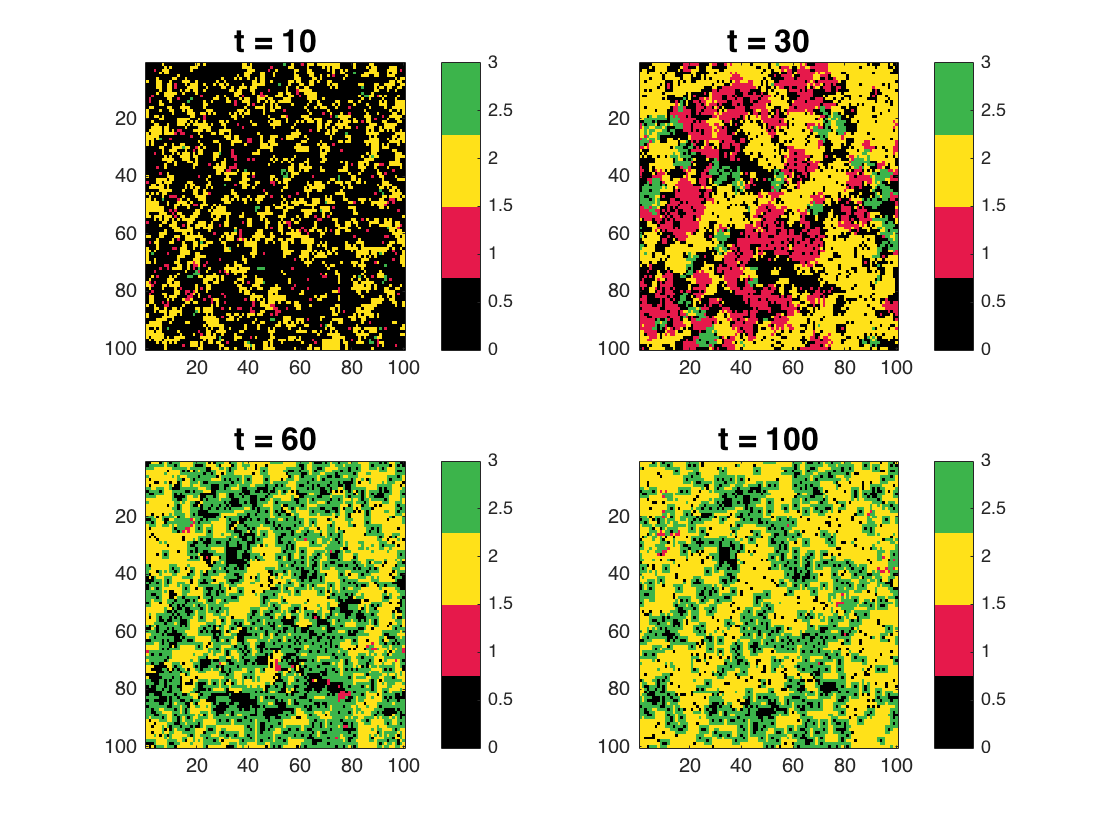
\includegraphics[scale=0.4]{Pictures/cInit.png}
    \caption{A grid of the cells at the systems initial state. Here the colors \{black, red, yellow, green\} correspond \{null, hunter, prey, hunterkiller\}}
    \label{fig:cInit}
\end{figure}              

\subsubsection{Usage of the defensive perimeter}  
In this section we initialize the system to have a blob of prey cells that are all inside a square of hunterkiller cells as seen in figure \ref{fig:square1}. A video can be found here.\footnote{https://vimeo.com/263157853} The progression of the system as the simulation is being run is seen in figure \ref{fig:square}. The growth of prey cells is contaminated to our initial defensive perimeter, with some small disfigurations. As the prey cells continue to grow/reproduce inside the square shaped structure they also become more prone to getting attacked by hunters, however the hunterkiller cells are always closeby and will defend the prey cells. This is partly seen in the subplot in figure \ref{fig:square} at timestep 90. 
   \begin{figure}[htbp]
    \centering
    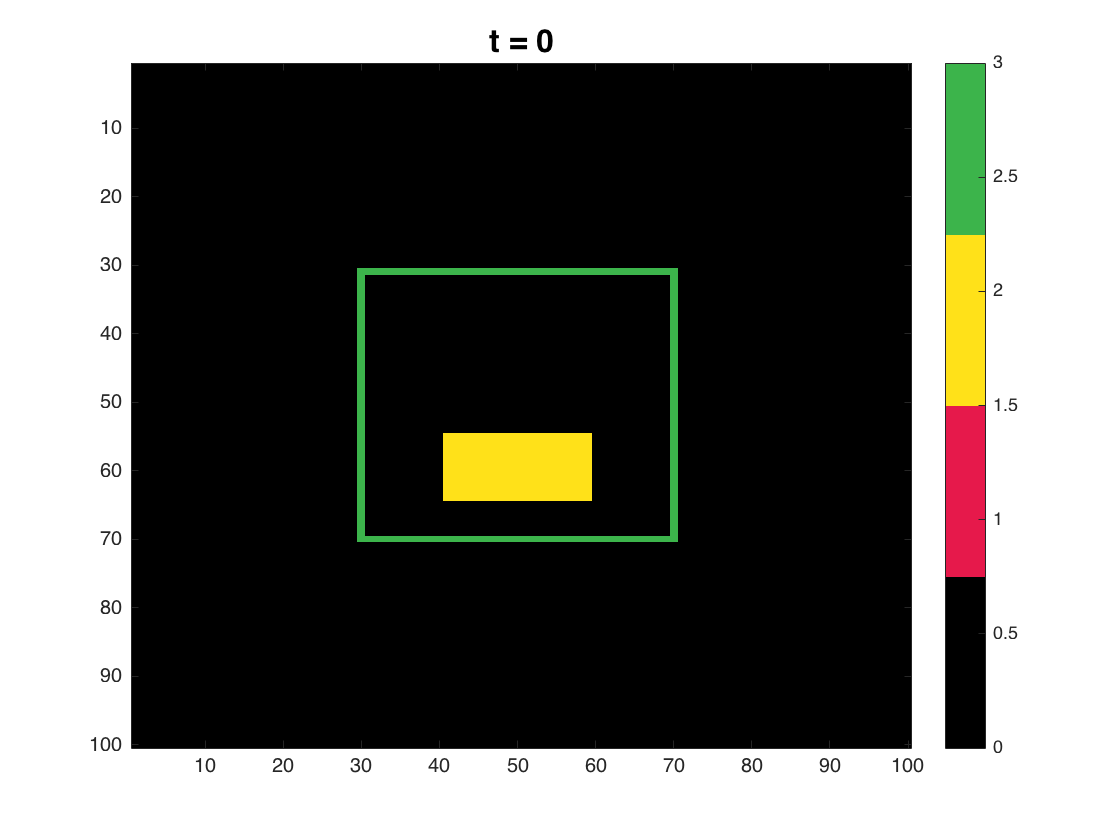
\includegraphics[scale=0.3]{Pictures/cSquare1.png}
    \caption{A bunch of prey cells inside a perimeter of hunterkiller cells}
    \label{fig:square1}
\end{figure}  
   \begin{figure}[htbp]
    \centering
    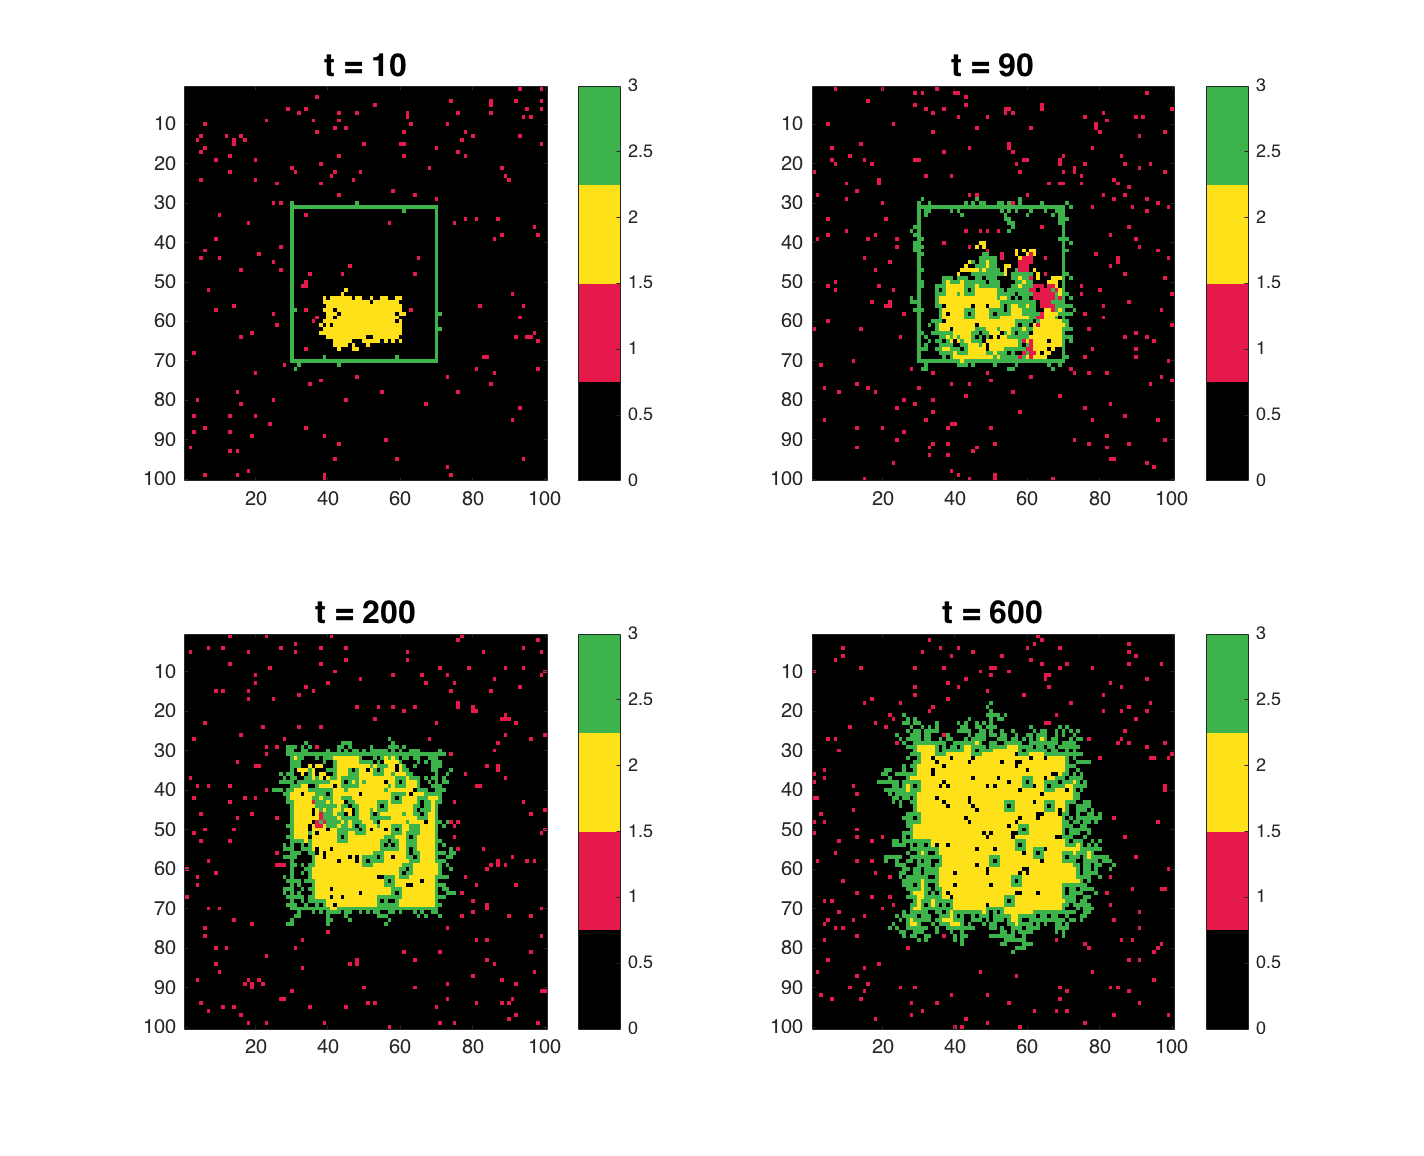
\includegraphics[scale=0.4]{Pictures/cSquare.png}
    \caption{The development of a system in which the initial state consisted of some prey cells inside a square-shaped perimeter of hunterkiller cells.}
    \label{fig:square}
\end{figure}    
We can see that at t = 600 almost all the hunterkiller cells are at the border of our initial structure, which is now slightly disfigured. This change of shapes come from the spawning of huntercells close to the border which in turns allows the growth of hunterkiller cells. Thus the \textit{hk} cells acts not only as a defensive parameter but also as a container of prey cells. 

\subsubsection{Prey or plague}
Let us now see what happens if we open up the top side of our square as seen in figure \ref{fig:bucket1}.\footnote{https://vimeo.com/263158853} Since there is no container of the prey cells as in the case above (see figure \ref{fig:square}) the prey cells spread uncontrollably throughout the system and after 600 timesteps nearly the whole system is covered in prey cells as seen in figure \ref{fig:bucket4}. 
     \begin{figure}[htbp]
    \centering
    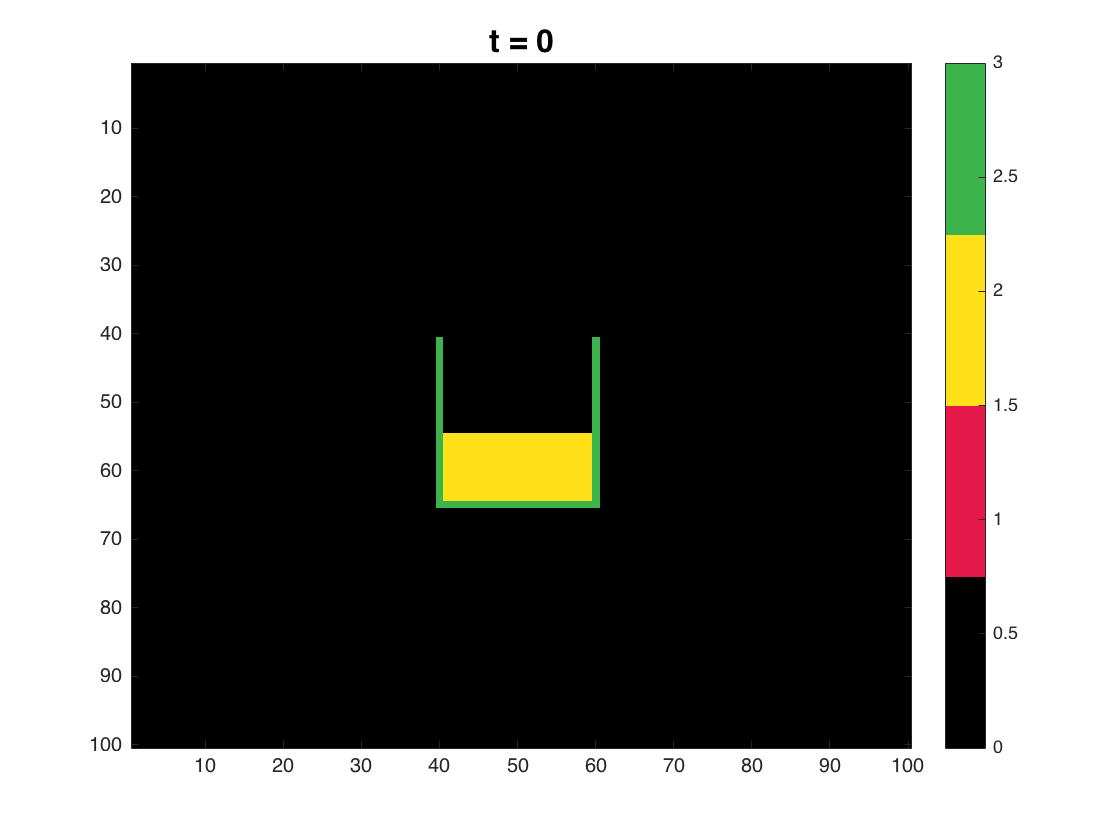
\includegraphics[scale=0.3]{Pictures/bucket1.png}
    \caption{A bunch of prey cells inside a "bucket" of hunterkiller cells}
    \label{fig:bucket1}
\end{figure}  

       \begin{figure}[htbp]
    \centering
    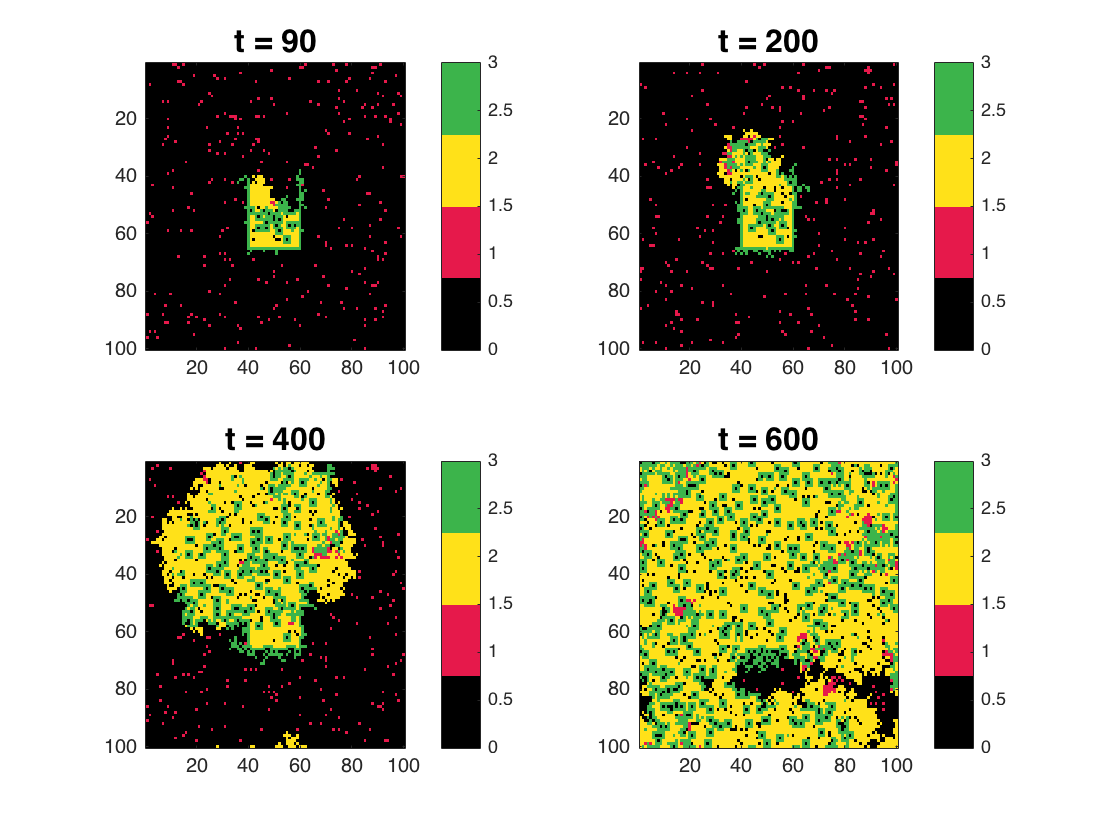
\includegraphics[scale=0.3]{Pictures/bucket4.png}
    \caption{The development of a system in which the initial state consisted of a bunch of prey cells inside a "bucket" of hunterkiller cells}
    \label{fig:bucket4}
\end{figure}  

\subsubsection{Conclusions regarding our costum system}
There are two ways in which we can reach something close to an equilibrium through the rules we have set. Either by letting the prey cells grow wildly and without imposing any constraints on them or by containing them within borders consisting of hunterkiller cells. In either case the hunter cells are set up to loose and will likely do so in almost all the cases. In a few percentage of the cases however, the system could end up in a state in which there are only hunter cells.
\section{Spread of memes}
In this part of the project we aim to simulate a simple model of how the spreading of memes takes places, or rather how people change their states (between the states resting, bored or sharing) when in contact with other people.
\subsection{A simple model}
The model is as follows: a person can be in one of three states \\ \\
\textbf{Resting}  With probability p a resting person will discover a new meme by herself and become a sharer \\
\textbf{Sharer}  With probability q a sharer will pick one person completely at random from the population. If that person is resting then she will now become a sharer. However, if the person she picks is bored, then the sharer will lose interest and become bored too. \\
\textbf{Bored} Bored people stay bored forever \\ \\

First we derive the mean field equations\\
\begin{align*}
R(t+1) & = R(t) - qR(t) - qS(t)\frac{R(t)}{1000}\\
B(t+1) & = B(t) + qS(t)\frac{B(t)}{1000}\\
S(t+1) & = S(t) + qR(t)+ qS(t)\frac{R(t)}{1000} - qS(t)\frac{B(t)}{1000}
\end{align*}
A simulation is run with 1000 people where, at the initial state, one is bored, one is sharing and the rest are resting. q = 0.01 and p = 0.001.
       \begin{figure}[htbp]
    \centering
    \includegraphics[scale=0.3]{Pictures/firstpart1.png}
    \caption{The number of sharers at different timesteps for simulations of the mean field equation and the average of a 1000 random simulations}
    \label{fig:fp}
\end{figure}  
The results of the implementation can be seen in figure \ref{fig:fp}. The mean field equation does a good job of describing the simulated average behavior of the model. It is only at the end that the two lines start to diverge. The random simulations are obtained by setting up a model which follows the rules of the system and simulating the outcome a thousand times for a thousand timesteps and finally taking the average of these outcomes.\\ \\
The reason to why the mean field equation diverges from the random simulations is could be that the random simulations become \textit{too} random towards the end. In figure \ref{fig:fp3} the mean field equation is plotted next to the graphs of all the random simulations. For the first 500 timesteps the random simulations form a relatively narrow band of lines whereas afterwards this band gets wider. The variance at the end is 60461, which is huge compared with the variance at timestep 300 which is 792.
       \begin{figure}[htbp]
    \centering
    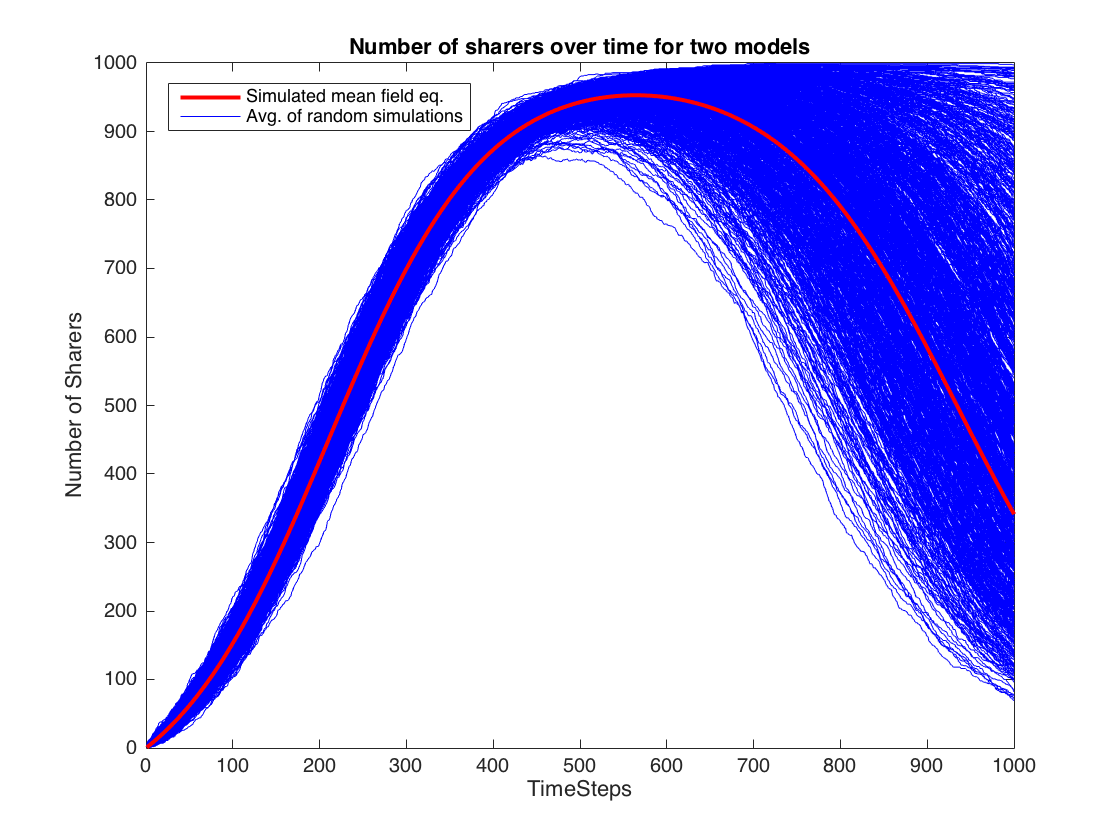
\includegraphics[scale=0.3]{Pictures/vargr.png}
    \caption{The number of sharers at different timesteps for simulations of the mean field equation and the average of a 1000 random simulations}
    \label{fig:fp3}
\end{figure}  
\subsubsection{Investigating the initial state}
We now turn to answer the question of how the initial number of bored people affects how well a meme does. In figure \ref{fig:fp4} the mean field equation with different amounts of initially bored people is plotted. From this graph it seems like looking at the amount of sharers at timestep 300 is a well-enough indicator of how "successful" will be (this allows us to decrease the length of the simulation and run it faster). It also seems like an increasingly amount of initially bored people will negatively impact the amount of sharers over time.  In figure \ref{fig:fp5} a phase transition plot show that this really is the behavior follows.\\
       \begin{figure}[htbp]
    \centering
    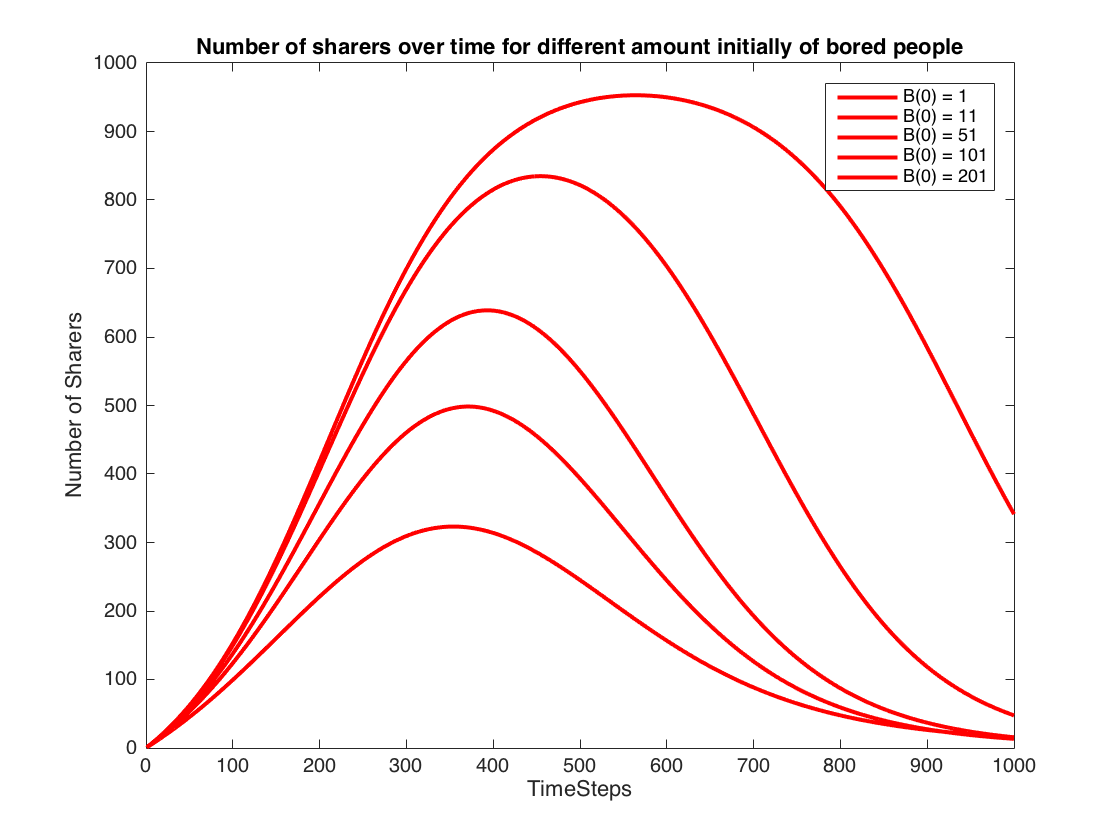
\includegraphics[scale=0.3]{Pictures/initbor.png}
    \caption{The number of sharers at different timesteps for the mean field equation with different initial amount of bored people.}
    \label{fig:fp4}
\end{figure}  
       \begin{figure}[htbp]
    \centering
    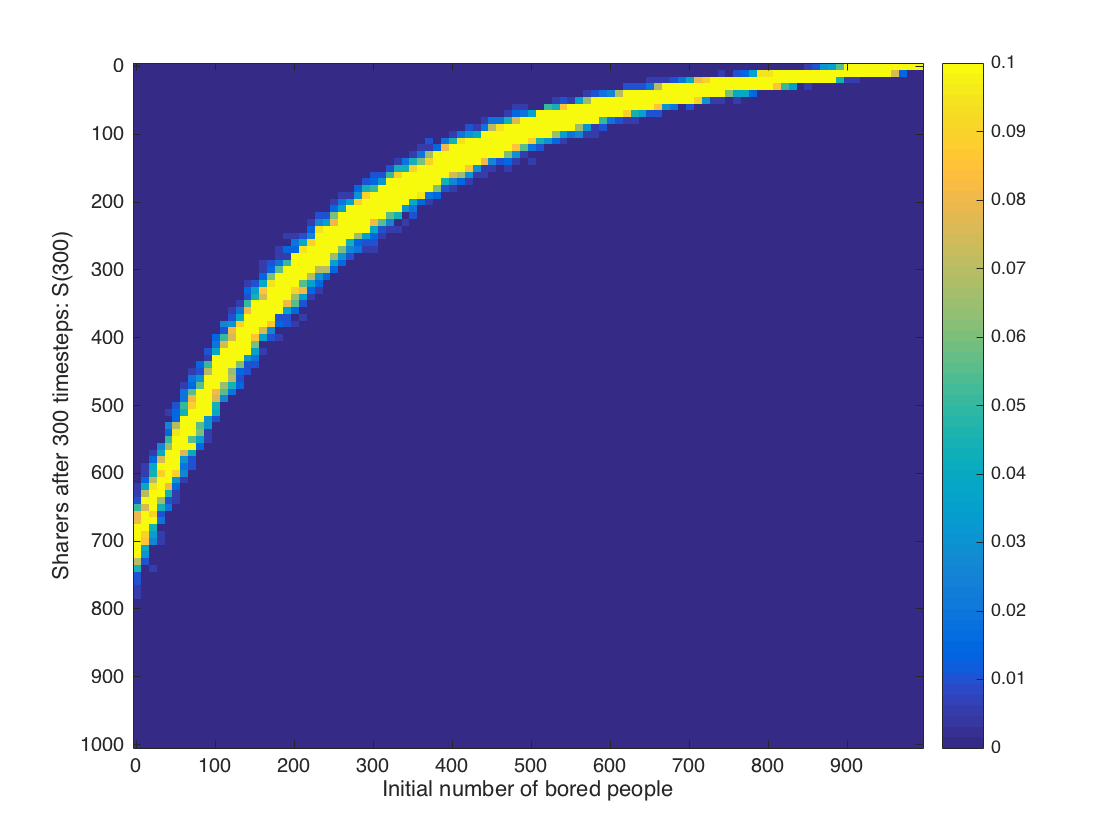
\includegraphics[scale=0.3]{Pictures/ptp.png}
    \caption{The number of sharers at different timesteps for the mean field equation with different initial amount of bored people. The initial number of bored people goes from 5 to 995 and is incremented by 5.}
    \label{fig:fp4}
\end{figure}  
\subsubsection{Probability of at least 25\% of the population sharing a meme}
Now we aim to find the probability of at least 25\% of the population sharing a meme \textbf{at the same time}. That means that (in our system) at a certain timestep 250 out of 1000 people should be sharers. We are not interested in the case were 125 people are sharing at one timestep and 125 completely different people are sharing at a different timestep. \\ The probability of this event can be approximated by simulating over different amounts of initially bored people and checking if there is any timestep in which the total amount of sharers are more than 250. A rough estimate is seen in figure \ref{fig:prob} in which 200 iterations have been run for each initial number of bored people B(0) Then for each B(0) the percentage of cases in which there has been 250 or more sharers at a timestep is plotted. For example, when $B(0) = 241$ then in 191 out of the 200 simulations there was a timestep in which the number of sharers exceeded 249.
       \begin{figure}[htbp]
    \centering
    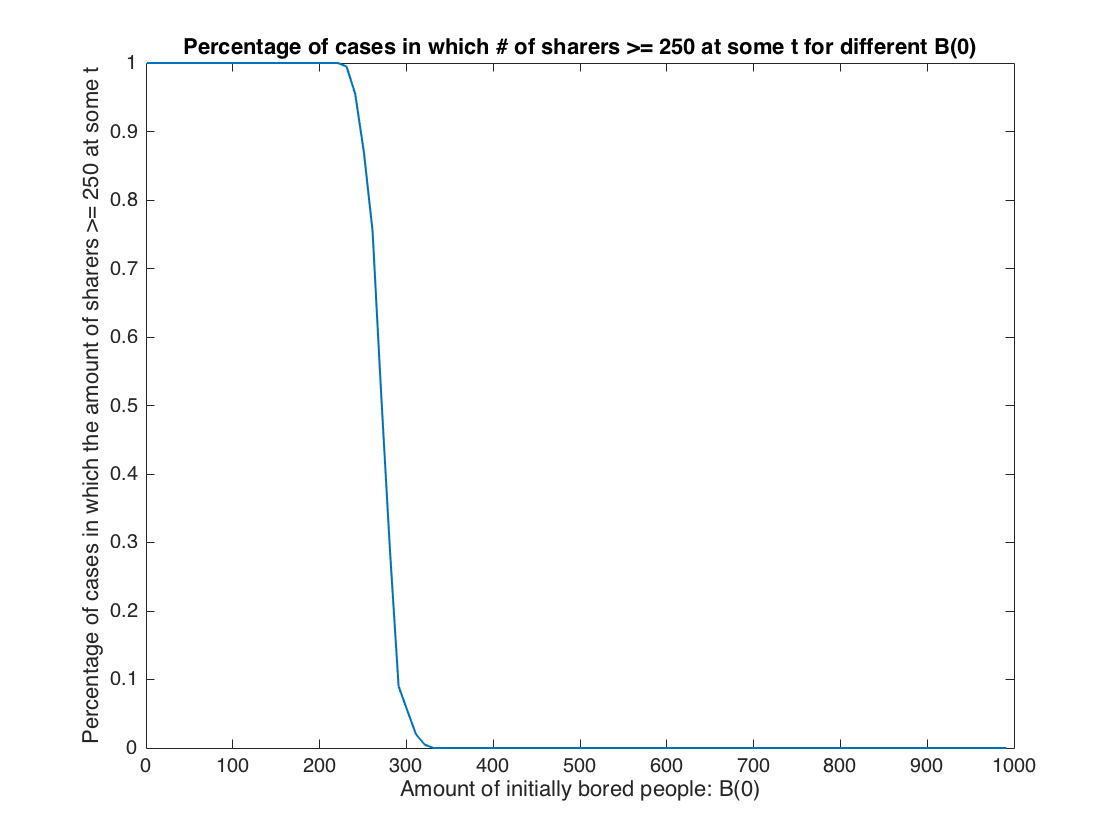
\includegraphics[scale=0.3]{Pictures/probg.png}
    \caption{The percentage of cases in which the number of sharers exceeded 249 for some timestep for different initial number of bored people. For each B(0), 200 simulations were run.}
    \label{fig:prob}
\end{figure}  
\subsection{Changing the model}
We now modify the model a little bit. The descriptions of the resting and sharer states remain the same, however we modify the bored state:\\ \\
\textbf{Bored} with probability q a bored person will pick one person completely at random from the population. If that person is resting then she will now become resting, otherwise she will continue to be bored. \\ \\
We use the amount of \{sharer, resting, bored\} = \{1, 989, 10\} and start by modifying q and look at how the system behaves. The simulations are run 100 iterations each and the results are seen in figure \ref{fig:aq1}. 
       \begin{figure}[htbp]
    \centering
    \includegraphics[scale=0.3]{Pictures/6eravg.png}
    \caption{The number of sharers at different timesteps for the mean field equation and the average of the simulations for different values of q. For each subplot there were 100 simulations. p = 0.001}
    \label{fig:aq1}
\end{figure}  
The mean field equation does a good job in estimating the outcome of the simulations when q is smaller than 0.01. In these cases the model seems to render a simple a \textit{simple} curve. However, as q is increased the mean field equation now shows an oscillating behaviour. It also starts to diverge from the results we obtain from our simulations, why is this? In figure \ref{fig:aq2} the result of the individual simulations are shown.
       \begin{figure}[htbp]
    \centering
    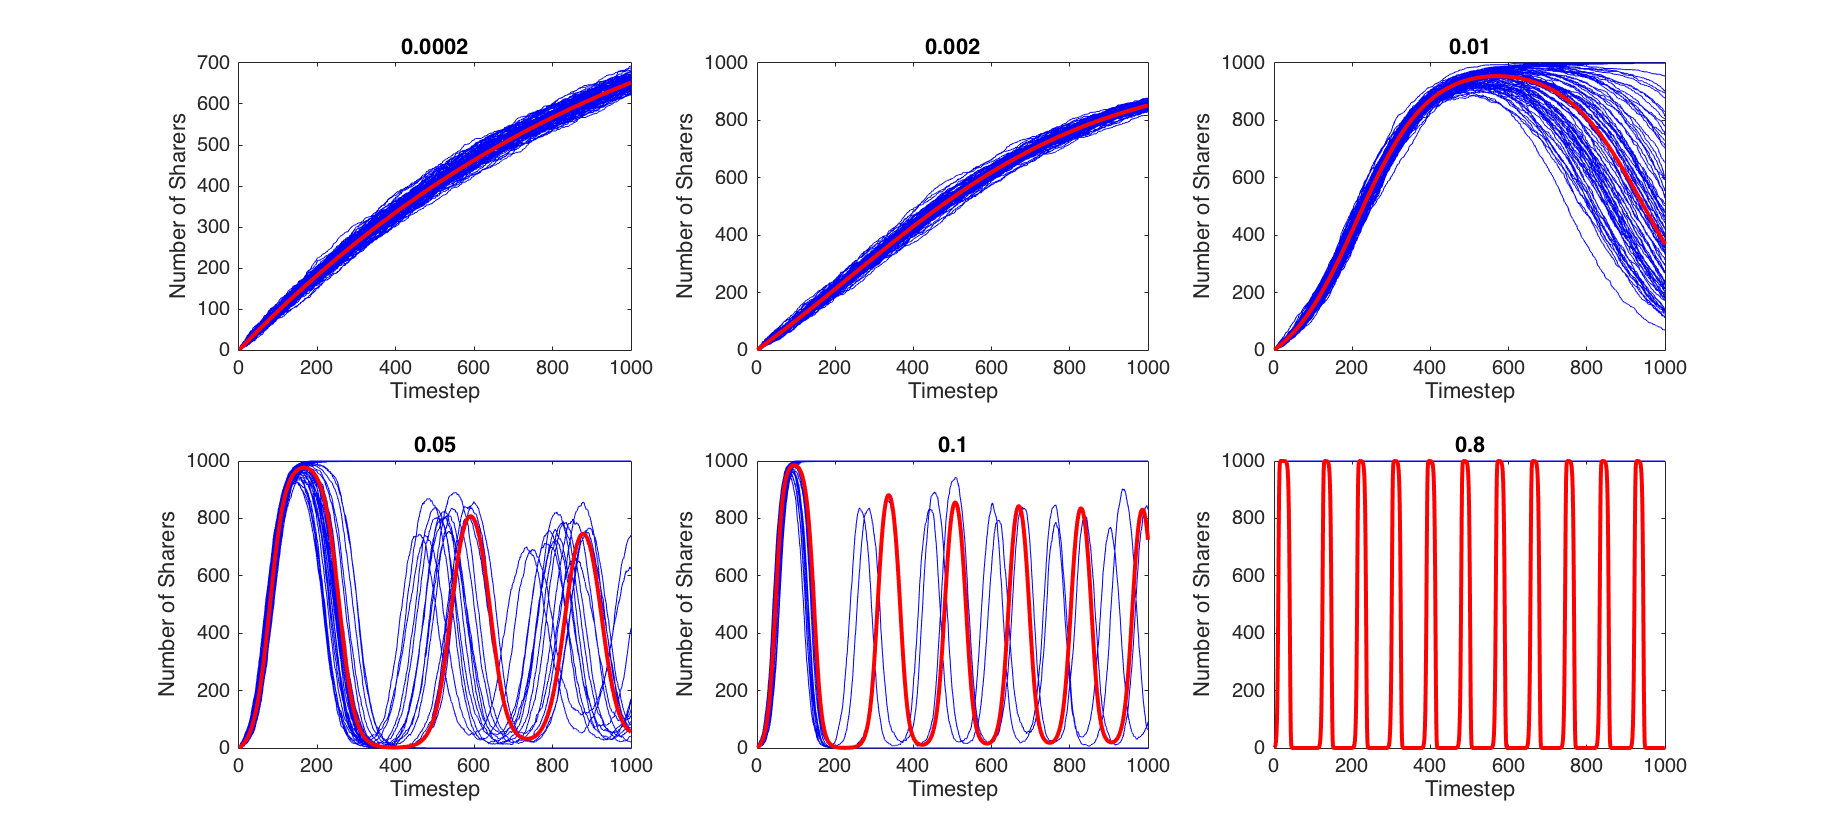
\includegraphics[scale=0.3]{Pictures/6er.png}
    \caption{The number of sharers at different timesteps for the mean field equation and of the simulations for different values of q. For each subplot there were 100 simulations. p = 0.001}
    \label{fig:aq2}
\end{figure}  
 We see that when q is less than or equal 0.01 all the simulations have the same behavior, even though they can diverge in their values, as the mean field equation. When q is larger than or equal to 0.05 it is seen that the simulations now have two different behaviors. Either the simulation follows the oscillating pattern described by the mean field equation or the amount of sharers settles at an extreme (0 or 1000).
 \subsubsection{1000 sharers}
In the case of 1000 sharers, there are neither any bored nor any resting people. Thus the amount of sharers cannot change since a sharer will pick a random person with probability q and this person will \textbf{always} be a sharer.
\subsubsection{0 sharers}
Having 0 sharers does not necessarily lead to a stagnation of the system (as is shown by some of the curves scratching the 0 line). However, this becomes a problem of the system also contains 0 resting people and only consists of bored people. In this case bored people with pick a random person with probability q and these persons will \textbf{always} be bored and will thus not lead to a different state of the system. \\ \\

Continuing, we now investigate how the system will behave when we change p. In figure \ref{fig:6p} the amount of sharers over time is plotted for different values of p (q = 0.01).
       \begin{figure}[htbp]
    \centering
    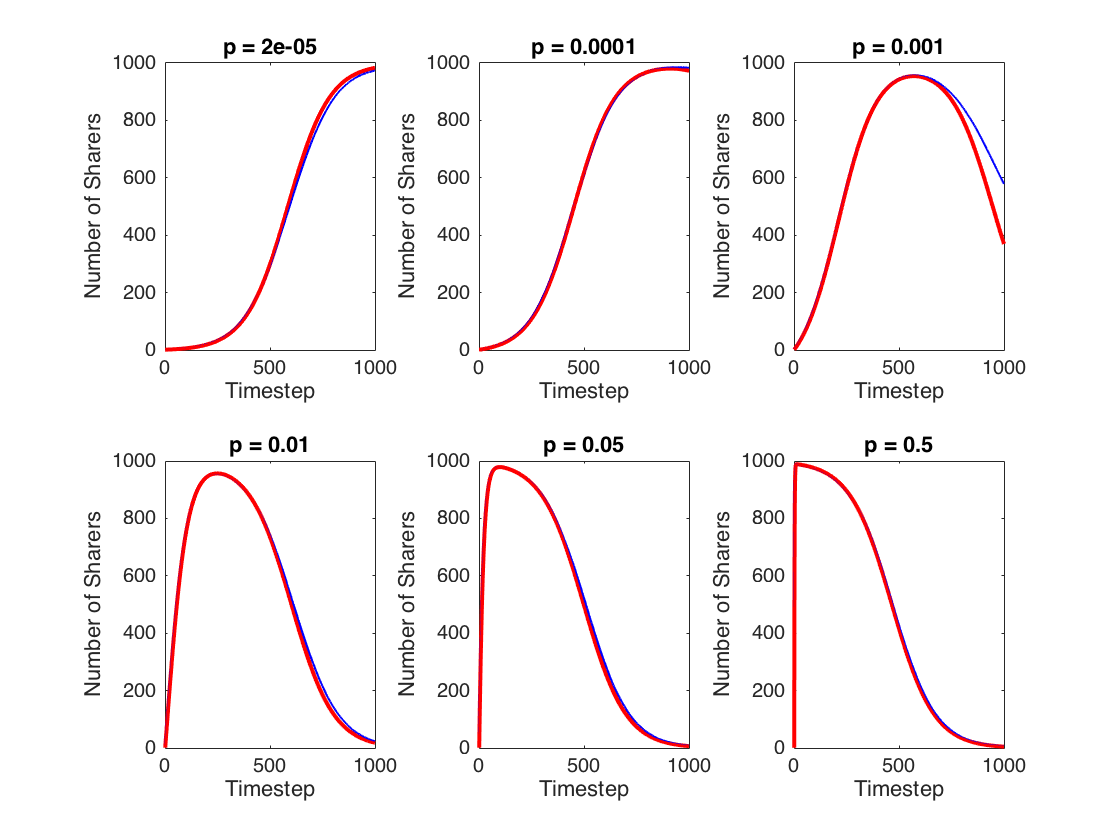
\includegraphics[scale=0.3]{Pictures/6averp.png}
    \caption{The number of sharers at different timesteps for the mean field equation and of the simulations for different values of p. For each subplot there were 100 simulations. q = 0.01}
    \label{fig:6p}
\end{figure}  
In this case, the mean field equation models the average behavior of the simulations really well over all the timesteps for all the different values of p. The behavior of the system however changes gradually for the different values. For the values of p that are smaller than 0.001 the number of sharers seem to increase and then \textit{settle} when they reach the end of the simulation. For the values of p larger or equal to 0.001 the number of sharers peaks before then end, after which its converges to zero. As we increase p, the peak occurs earlier. The variable p can thus be described as the eagerness to become a sharer of a resting person and if the population of resting persons are too eager we see that in the end we will have very few sharers since they all become bored.\\ \\
\subsection{Simulation with cells}
We now implement the system on a 2D grid as in the first part of this report. We will use the same model as we just used with the difference that a person only interact with the neighboring persons (or cells), that is the 8 surrounding persons. The color-scheme used in the simulations are \{bored, resting, sharing\} correspond to the colors \{red, yellow, black\}.\\ \\
We start of by implementing the same model as earlier with 5 bored people on a 32x32 grid (1024 people).\footnote{First implementation: https://vimeo.com/263896039} Since the amount of bored people are so few and they are usually surrounded by resting people there is a relatively high probability of them becoming resting (the probability for a bored person that is completely surrounded by resting people is q = 0.01.). This will give us a system of only resting/sharing people which in turn will result in a system of only sharing people. In order to circumvent this pattern we increase the initial number of bored people. \footnote{50 bored people: https://vimeo.com/263894083} Now it is far more likely that some bored people will remain bored as the system develops.\\ \\ The system seems to develop fairly slowly, let us try to to see what happens if we increase the value of q to 0.05. In the previous part (see figure \ref{fig:aq2}) this led to an oscillating behavior or a stationary system. These states are also captured in the grid implementation as seen in the videos. \footnote{All bored end state: https://vimeo.com/263914390}\footnote{All sharing end state: https://vimeo.com/263914388}\footnote{More equal end state: https://vimeo.com/263914364} In the last video the sharers first become a heavy majority and then being overtaken by bored people and finally resulting in a more balanced distribution of people (\{bored, resting, sharing\} = \{373, 284, 367\}). \\�\\
When increasing the value of p to 0.1 we one again have the occurrence of an early peak followed by a decline in the amount of sharers. \footnote{Early peak of sharers: https://vimeo.com/263922463}
\newpage
\begin{appendix}{Appendix code for part A}\\ \\
Main function
 \begin{lstlisting}
close all
clear all

N = 100;


%Initialize the matrix and randomly set the value to 0 (ready), 1(firing)
%or 2(resting).

Pread = 0.3;    %Probability of being in firing state

B_ar = zeros(N,N);
B_temp = zeros(N,N);
for i = 1:1:N
    for j = 1:1:N
        z = rand;
        if (z <Pread)
            B_ar(i,j) = 1;
        else
            B_ar(i,j) = 0;
        end
    end
end
imagesc(B_ar);
caxis([0 2]);
colorbar;
title(['\fontsize{16}t = 0']);
%At each timestep, check the neighbours and determine a new state
%for each state
r = 1;

for t = 1:1000
    
    for i = 1:1:N
        for j = 1:1:N
            B_temp(i,j) = newState(B_ar, i, j);
        end
    end
    B_ar = B_temp;
    %if (t == 10 || t == 20 || t == 100 || t == 1000)
    %    k = waitforbuttonpress;
    %    if k == 1
    %        error('Stopped');
    %    end
    pause(0.5)
    r = r+1
    
    imagesc(B_ar);
    caxis([0 2]);
    colorbar;
    title(['\fontsize{16}t = ', num2str(t)]);
    
    %end
    
    
end
\end{lstlisting}
newState.m \qquad Function for determining new state
\begin{lstlisting}
function B=newState(A, i, j)
N = size(A,1);
if (A(i,j) == 1 || A(i,j) ==2)                  %Check if it is a firing
    B = mod((A(i,j)+1), 3);                     %or resting cell
else
    if (i == j && i == 1)
        Neighbours = [A(i+1,j); A(i,j+1); A(N,1); A(1,N); A(i+1,j+1); A(N,j+1); A(i+1, N); A(N,N)];
    elseif (i == 1)
        Neighbours = [A(i+1,j); A(i,mod(j,N)+1); A(N, j); A(i,j-1); A(i+1,j-1); A(N, j-1); A(i+1,mod(j,N)+1); A(N,mod(j,N)+1)];
    elseif (j == 1)
        Neighbours = [A(mod(i,N)+1,j); A(i,j+1); A(i-1, j); A(i,N); A(mod(i,N)+1,j+1); A(mod(i,N)+1,N); A(i-1,j+1);A(i-1,N)];
    else
        Neighbours = [A(mod(i,N)+1,j); A(i-1,j); A(i,mod(j,N)+1); A(i,j-1); A(mod(i,N)+1,j-1); A(i-1, j-1); A(i-1, mod(j,N)+1); A(mod(i,N)+1,mod(j,N)+1) ];
    end
    Num_firing = sum(Neighbours == 1);
    if (i == 10 && j == 9)
        Neighbours
    end
    if (Num_firing == 2)
        B = 1;
    else
        B = 0;
    end
end
\end{lstlisting}

Count function
\begin{lstlisting}
function B=newState(A, i, j)
N = size(A,1);
if (A(i,j) == 1 || A(i,j) ==2)                  %Check if it is a firing
    B = mod((A(i,j)+1), 3);                     %or resting cell
else
    if (i == j && i == 1)
        Neighbours = [A(i+1,j); A(i,j+1); A(N,1); A(1,N); A(i+1,j+1); A(N,j+1); A(i+1, N); A(N,N)];
    elseif (i == 1)
        Neighbours = [A(i+1,j); A(i,mod(j,N)+1); A(N, j); A(i,j-1); A(i+1,j-1); A(N, j-1); A(i+1,mod(j,N)+1); A(N,mod(j,N)+1)];
    elseif (j == 1)
        Neighbours = [A(mod(i,N)+1,j); A(i,j+1); A(i-1, j); A(i,N); A(mod(i,N)+1,j+1); A(mod(i,N)+1,N); A(i-1,j+1);A(i-1,N)];
    else
        Neighbours = [A(mod(i,N)+1,j); A(i-1,j); A(i,mod(j,N)+1); A(i,j-1); A(mod(i,N)+1,j-1); A(i-1, j-1); A(i-1, mod(j,N)+1); A(mod(i,N)+1,mod(j,N)+1) ];
    end
    Num_firing = sum(Neighbours == 1);
    if (i == 10 && j == 9)
        Neighbours
    end
    if (Num_firing == 2)
        B = 1;
    else
        B = 0;
    end
end
\end{lstlisting}
\end{appendix}
\begin{appendix}{Appendix code for part B}\\ \\
Main function
 \begin{lstlisting}
 % In this program the cells can be in four different states;
% null (0), hunter(1), prey(2) and hunter-killer(3).
% A null cell can turn into a null cell if it has two or more neighbouring
% prey-cells.
% A hunter turn into a hunter-killer if it is neighbours a hunter-killer.
% A prey turn into a hunter if it is surrounded by hunters and non-null
% cells (nowhere to escape). At any moment a prey can move into a null-cell
% unless with a certain probability p. This probability is reduced as the
% amount of hunter neighbours increase.

function y = Cprogram(inp)
close all
N = 100;


%Initialize the matrix and randomly set the value to 0(60%), 1(5%), 2(30%) or 3(5%).

Pread = 0.3;    %Probability of being in firing state

B_ar = zeros(N,N);
B_temp = zeros(N,N);

if strcmpi(inp, 'foundation')
    %B_ar(:,50) = 2;
    B_ar(50,:) = 2;
    B_ar(51,:) = 3;
elseif strcmpi(inp, 'seeds')
    for i = 1:1:5
        for j = 1:1:5
            B_ar(10+i,10+j) = 2;
            B_ar(40+i,40+j) = 2;
        end
    end
    B_ar(13,13) = 3;
    B_ar(43,43) = 3;
    
elseif strcmpi(inp, 'bucket')
    for i = 1:1:25
        B_ar(40+i,40) = 3;
        B_ar(40+i,60) = 3;
    end
    for l = 1:1:20
        B_ar(65, 40+l) = 3;
    end
    for l = 1:1:10
        for i = 1:1:19
            B_ar(54+l, 40+i) = 2;
        end
        
    end
elseif strcmpi(inp, 'square')
    for i = 1:1:40
        B_ar(30+i,30) = 3;
        B_ar(30+i,70) = 3;
    end
    for l = 1:1:40
        B_ar(31, 30+l) = 3;
        B_ar(70, 30+l) = 3;
    end
    for l = 1:1:10
        for i = 1:1:19
            B_ar(54+l, 40+i) = 2;
        end
        
    end
    
else
    for i = 1:1:N
        for j = 1:1:N
            z = rand;
            if (z < 0.90)
                B_ar(i,j) = 0;
            elseif (z < 0.975)
                B_ar(i,j) = 2;
            elseif (z < 0.995)
                B_ar(i,j) = 1;
            else
                B_ar(i,j) = 3;
            end
        end
    end
end
mymap = [0 0 0
    230 25 75
    255 225 25
    60 180 75]/255;

imagesc(B_ar);
colormap(mymap);
caxis([0 3]);
colorbar;
title(['\fontsize{16}t = 0']);
figure
%At each timestep, check the neighbours and determine a new state
%for each state
r = 1;
        k = waitforbuttonpress;
        if k == 1
            error('Stopped');
        end

for t = 1:1000
    t
    for i = 1:1:N
        for j = 1:1:N
            B_temp(i,j) = newStateC(B_ar, i, j);
        end
    end
    B_ar = B_temp;
%     if (t == 90 || t == 200 || t == 400 || t == 600)
%         k = waitforbuttonpress;
%         if k == 1
%             error('Stopped');
%         end
%         subplot(2,2,r);
        
        r = r+1
        imagesc(B_ar);
        colormap(mymap);
        caxis([0 3]);
        colorbar;
        title(['\fontsize{16}t = ', num2str(t)]);
        drawnow
        pause(0.004)
% end
    
    
end
end
\end{lstlisting}
Count.m
\begin{lstlisting}
function r=count(A, i, j, state)
r = 0;
N = size(A,1);

if (j == 1)
    left = N;
    right = 2;
elseif (j == N)
    left = N-1;
    right = 1;
else
    left = j-1;
    right = j+1;
end

if (i == 1)
    up = N;
    down = 2;
elseif (i == N)
    up = N-1;
    down = 1;
else
    up = i-1;
    down = i+1;
end


if (A(up,left) == state)
    r = r+1;
end
if (A(up,j) == state)
    r = r+1;
end
if (A(up,right) == state)
    r = r+1;
end
if (A(i,left) == state)
    r = r+1;
end
if (A(i,right) == state)
    r = r+1;
end
if (A(down,left) == state)
    r = r+1;
end
if (A(down,j) == state)
    r = r+1;
end
if (A(down,right) == state)
    r = r+1;
end

end
\end{lstlisting}
Count2.m
\begin{lstlisting}
function [r,t]=count2(A, i, j, state1,state2)
r = 0;
t = 0;
N = size(A,1);


if (j == 1)
    left = N;
    right = 2;
elseif (j == N)
    left = N-1;
    right = 1;
else
    left = j-1;
    right = j+1;
end

if (i == 1)
    up = N;
    down = 2;
elseif (i == N)
    up = N-1;
    down = 1;
else
    up = i-1;
    down = i+1;
end


if (A(up,left) == state1)
    r = r+1;
elseif (A(up,left) == state2)
    t = t+1;
end

if (A(up,j) == state1)
    r = r+1;
elseif (A(up,j) == state2)
    t = t+1;
end

if (A(up,right) == state1)
    r = r+1;
elseif (A(up,right) == state2)
    t = t+1;
end

if (A(i,left) == state1)
    r = r+1;
elseif (A(i,left) == state2)
    t = t+1;
end

if (A(i,right) == state1)
    r = r+1;
elseif (A(i,right) == state2)
    t = t+1;
end

if (A(down,left) == state1)
    r = r+1;
elseif (A(down,left) == state2)
    t = t+1;
end

if (A(down,j) == state1)
    r = r+1;
elseif (A(down,j) == state2)
    t = t+1;
end

if (A(down,right) == state1)
    r = r+1;
elseif (A(down,right) == state2)
    t = t+1;
end

end
\end{lstlisting}
newState.m
\begin{lstlisting}
% In this program the cells can be in four different states;
% null (0), hunter(1), prey(2) and hunter-killer(3).
% A null cell can turn into a prey cell if it has a neighbouring
% prey-cells and no neighbouring hunter cells. It can also turn into a
% hunter cell with a some probability.
% A hunter turn into a hunter-killer if it is neighbours a hunter-killer or
% it can turn into a null cell with some probability.
% A prey turn into a hunter if it is surrounded by hunters and non-null
% cells (nowhere to escape). At any moment a prey can move into a null-cell
% unless with a certain probability p. This probability is reduced as the
% amount of hunter neighbours increase.

%Parameters:
%Probability matrix of Null => prey: [0 5 7.5 10 12.5 15 17.5 20]


function B=newState(A, i, j)
B = (A(i,j));
N = size(A,1);
z = rand;
if (A(i,j) == 0)                  %If null cell
    Null_to_pray = [0 3 6 9 12 16 20 25 30]/100;
    Null_to_hunt = [3 3 3 2 2 2 1 1 1]/1000;
    [amount_of_prey, amount_of_hunter] = count2(A, i, j, 2, 1);
    if ~(amount_of_hunter) && (Null_to_pray(amount_of_prey+1) > z)
        B = 2;
    elseif  (Null_to_hunt(amount_of_hunter+1) > z)
        B = 1;
    end
elseif (A(i,j) == 1)            %If hunter cell
    [amount_of_hk, amount_of_null] = count2(A, i, j, 3, 0);
    Hunt_to_hk = [0.5 0.75 0.8 0.9 0.95 1 1 1];   
    if (amount_of_hk && Hunt_to_hk(amount_of_hk) > z)
        B = 3;
    elseif (z < 0.001)
        B = 0;
    elseif (amount_of_null >= 6 && z < 0.10)
        B = 0;
    end
elseif (A(i,j) == 2)            %Prey cell
    [amount_of_hunter, amount_of_null] = count2(A, i, j, 1, 0);
    amount_of_prey = count(A, i, j, 2);
    perc_of_null = amount_of_null/8;
    Prey_to_hunter = [0.3 0.4 0.5 0.6 0.7 0.8 0.9 1]*(1-perc_of_null);   
    if (amount_of_hunter) && (Prey_to_hunter(amount_of_hunter)>z)
        B = 1;
    elseif (amount_of_hunter) && (0.02>z)
        B = 3;
    elseif (amount_of_prey == 8) && (z < 0.02)
        %B = 1;
    elseif (z <0.03 && amount_of_prey > 5 && amount_of_hunter == 0)
        B = 0;
    end
elseif (A(i,j) == 3)
    [amount_of_hk, amount_of_prey] = count2(A, i, j, 3, 2);
    amount_of_hunter = count(A, i, j, 1);
    if ((amount_of_hk + amount_of_prey) == 8) && z<0.3     %If completely surrounded by "friendly" cells
        B = 2;
    elseif (z<0.02 && ~(amount_of_hunter))  %Defence deteriorating
        %B = 2;
    end
end

\end{lstlisting}
\end{appendix}
\begin{appendix}{project 2}
\\ Sharing of memes SoM.m
\begin{lstlisting}
% Three states: resting (0), bored(1) and sharer (2)

clear all
close all

N = 1000;
p = 0.001;
q = 0.01;
Iter = 1000;
TimeSteps= 1000;


NumOfSharers = zeros(1, Iter);
NumOfBored = zeros(1, Iter);
NumOfSharersTot = zeros(TimeSteps, Iter);
%%Mean field equation simulation
X = 1;  %Sharers
Y = 998; %Resting
Z = 1; %Bored
for t = 1:1:TimeSteps-1
    t1 = Y(t)*p;
    t2 = q*X(t)*Y(t)/1000;
    t3 = q*X(t)*Z(t)/1000;
    X(t+1) = X(t) + t1 + t2 - t3;
    Y(t+1) = Y(t)- t1 - t2;
    Z(t+1) = Z(t) + t3;
end
plot(1:1:1000, X, 'r', 'LineWidth', 2);
hold on

for j = 1:1:1000
    People = zeros(1, N);
    for l = 1:1:1
        People(l) = 1;
    end
    
    temp = randi(N);
    while (People(temp) == 1)
        temp = randi(N);
    end
    People(temp) = 2;
    PeopleTemp = People;
    
    for t = 1:1:TimeSteps
        for i = 1:1:N
            if (People(i) == 0)     %resting
                if (p > rand)
                    PeopleTemp(i) = 2;
                end
            elseif (People(i) == 2) %sharer
                if (q > rand)
                    temp = randi(N);
                    while (temp == i)
                        temp = randi(N);
                    end
                    if (People(temp) == 1)
                        PeopleTemp(i) = 1;
                    else
                        PeopleTemp(temp) = 2;
                        PeopleTemp(i) = 2;
                    end
                end
            end
        end
        People = PeopleTemp;
        NumOfSharersTot(t, j) = sum(People==2);
    end
        plot(1:1:TimeSteps, NumOfSharersTot(:,j), 'b');
        hold on
        drawnow
        %NumOfSharers(j) = sum(People == 2);
        NumOfBored(j) = sum(People == 1);
        NumOfSharersTot(j,t)
end

% plot(1:1:TimeSteps, mean(NumOfSharersTot,2), 'b', 'LineWidth', 2);
% hold on
% drawnow
%%NumOfSharers(j) = sum(People == 2);




%plot(1:1:Iter,NumOfSharers, 'LineWidth', 2);
xlabel('TimeSteps', 'FontSize', 16);
ylabel('Number of Sharers', 'FontSize', 16);
legend('Simulated mean field eq.', 'Avg. of random simulations');
title('Number of sharers over time for two models')
\end{lstlisting}
Number of shared NumOfShar.m
\begin{lstlisting}
% Three states: resting (0), bored(1) and sharer (2)

function S = NumOfSharMax(B)
N = 1000;
p = 0.001;
q = 0.01;
Iter = 1000;
TimeSteps= 650;


NumOfSharers = zeros(1, Iter);
NumOfBored = zeros(1, Iter);
NumOfSharersTot = zeros(TimeSteps, Iter);
% %%Mean field equation simulation
% X = 1;  %Sharers
% Y = 998; %Resting
% Z = 1; %Bored
% for t = 1:1:TimeSteps-1
%     t1 = Y(t)*p;
%     t2 = q*X(t)*Y(t)/1000;
%     t3 = q*X(t)*Z(t)/1000;
%     X(t+1) = X(t) + t1 + t2 - t3;
%     Y(t+1) = Y(t)- t1 - t2;
%     Z(t+1) = Z(t) + t3;
% end
% plot(1:1:1000, X, 'r', 'LineWidth', 2);
% hold on 

for j = 1:1:1
    People = zeros(1, N);
    for l = 1:1:B
        People(l) = 1;
    end
    
    temp = randi(N);
    while (People(temp) == 1)
        temp = randi(N);
    end
    
    People(temp) = 2;
    PeopleTemp = People;
    
    for t = 1:1:TimeSteps
        for i = 1:1:N
            if (People(i) == 0)     %resting
                if (p > rand)
                    PeopleTemp(i) = 2;
                end
            elseif (People(i) == 2) %sharer
                if (q > rand)
                    temp = randi(N);
                    while (temp == i)
                        temp = randi(N);
                    end
                    if (People(temp) == 1)
                        PeopleTemp(i) = 1;
                    else
                        PeopleTemp(temp) = 2;
                        PeopleTemp(i) = 2;
                    end
                end
            end
        end
        People = PeopleTemp;
        NumOfSharersTot(t, j) = sum(People==2);
    end
    %%NumOfSharers(j) = sum(People == 2);
    NumOfBored(j) = sum(People == 1);
    S = max(NumOfSharersTot(:,1));
    %plot(1:1:TimeSteps, NumOfSharersTot(:,j), 'b');

end
end




\end{lstlisting}
RunNOS.m
\begin{lstlisting}
%Set up paremater values
rvals=[1:10:995]
numreps=200;
hrange=[0:10:1000];
histS=zeros(length(rvals),length(hrange));


% Simulate numreps times for each parameter setting
count=0;
for r=rvals
    r
    uall=[];
    count=count+1

    for rep=1:numreps
        S=NumOfSharMax(r);
        finalS(count,rep)=S(end);
    end
end

p = max(finalS,2);
\end{lstlisting}
Cells.m
\begin{lstlisting}
close all
clear all

N = 32;


%Initialize the matrix and randomly set the value to 0 (resting), 1(bored)
%or 2(sharer).

B_ar = zeros(N,N);
B_temp = zeros(N,N);

%10 initially bored ones
i = randi(N);
j = randi(N);

for l = 1:1:50
    while (B_ar(i,j) == 1)
        i = randi(N);
        j = randi(N);
    end
    B_ar(i,j) = 1;
end

while(B_ar(i,j) == 1)
    i = randi(N);
    j = randi(N);
end
B_ar(i,j) = 2;
mymap = [0 0 0
   230 25 75
   255 225 25]/255;
imagesc(B_ar);
colormap(mymap);
caxis([0 2]);
colorbar;
title(['\fontsize{16}t = 0']);
B_temp = B_ar;
%At each timestep, check the neighbours and determine a new state
%for each state
r = 1;
figure
k = waitforbuttonpress;
if k == 1
    error('Stopped');
end
for t = 1:1:1000
    for i = 1:1:N
        for j = 1:1:N
            B_temp = newState(B_temp, i, j);
        end
    end
    B_ar = B_temp;
    %if (t == 10 || t == 20 || t == 100 || t == 1000)
    %    k = waitforbuttonpress;
    %    if k == 1
    %        error('Stopped');
    %    end
    pause(0.005)
    r = r+1;
    
    imagesc(B_ar);
    colormap(mymap);
    caxis([0 2]);
    colorbar;
    title(['\fontsize{16}t = ', num2str(t)]);
    drawnow
    %end
    
    
end

\end{lstlisting}
newState.m
\begin{lstlisting}
%The input should be reimplemented to be a 3x3 array.

function B=newState(A, i, j)
B = A;
N = size(A,1);
p = 0.001;
q = 0.03;
r = q;%r = 0.0001;
if (j == 1)
    left = N;
    right = 2;
elseif (j == N)
    left = N-1;
    right = 1;
else
    left = j-1;
    right = j+1;
end

if (i == 1)
    up = N;
    down = 2;
elseif (i == N)
    up = N-1;
    down = 1;
else
    up = i-1;
    down = i+1;
end

Neighbors = [A(up, left) A(up, j) A(up, right) A(i, left) A(i, right) A(down, left) A(down, j) A(down, right)];
if (A(i,j) == 0)    %If its a resting cell, no interaction
    if (p > rand)
       B(i,j) = 2;
    end
elseif (A(i,j) == 1)    %if its a bored cell
    if (r > rand && Neighbors(randi(8)) == 0)
            B(i,j) = 0;
    end
else
    if (q > rand)
        num = randi(8);
        MyN =  Neighbors(num);
        if (MyN == 0)
            Neighbors(num) = 2;
            
            B(up, left) = Neighbors(1);
            B(up, j)= Neighbors(2);
            B(up, right)= Neighbors(3);
            B(i, left) = Neighbors(4);
            B(i, right) = Neighbors(5);
            B(down, left)= Neighbors(6);
            B(down, j)= Neighbors(7);
            B(down, right)= Neighbors(8);
        elseif (MyN == 1)
            B(i,j) = 1;
        end
    end
end
end
\end{lstlisting}
\end{appendix}
\end{document}
              